\paragraph{Empty cells that override column fills.}
An additional Enron case illustrates a visible fill change (Figure~\ref{fig:enron-fill-override}). Check Performance removes empty cells with an explicit gray fill, exposing the pink fill inherited from their columns. On \texttt{PL-Consolidated}, 190,872 such cells occur below the last populated row. Excel Shrink Default retains these overrides because deleting them changes the displayed background.

We copied the converted original and both outputs, ran \texttt{CalculateFullRebuild} in Excel 16.0 build 20326, waited for calculation to complete and saved each copy. External links were not refreshed. Earlier stale-value strikethroughs disappeared, while the background difference remained. Original and Default captures were pixel-identical in both inspected regions, \texttt{PL-Consolidated!A25:H37} and \texttt{PL-Houston!A30:H42}. The latter region is included in the supplementary case files.

\begin{figure*}[t]
\centering
\subfigure[Converted original]{
\includegraphics[width=0.90\textwidth]{figures/case-studies/enron-fill-override/Original--PL-Consolidated-boundary.png}}
\par
\subfigure[Excel Shrink Default]{
\includegraphics[width=0.90\textwidth]{figures/case-studies/enron-fill-override/Default--PL-Consolidated-boundary.png}}
\par
\subfigure[Check Performance after Optimize All]{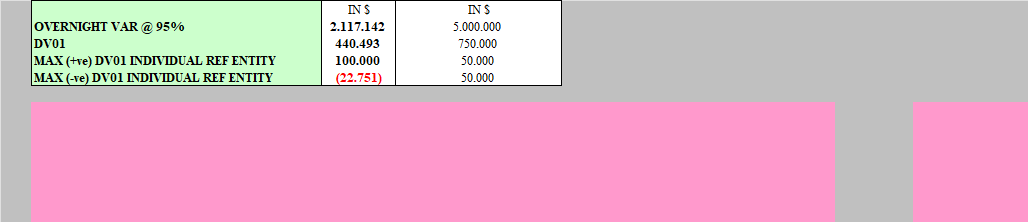
\includegraphics[width=0.90\textwidth]{figures/case-studies/enron-fill-override/Check-Performance--PL-Consolidated-boundary.png}}
\par
\caption{Enron fill overrides after full rebuild and Save. All three captures show PL-Consolidated!A25:H37. Check Performance exposes pink column formatting below the populated rows. Excel Shrink preserves the original gray background.}
\label{fig:enron-fill-override}
\end{figure*}
